\documentclass[11pt]{article}
\usepackage[a4paper, margin=2.54cm]{geometry}
\usepackage[utf8]{inputenc}
\usepackage[spanish, mexico]{babel}
\usepackage[spanish]{layout}
\usepackage{amsmath}
\usepackage{amssymb}
\usepackage{amsfonts}
\usepackage{tikz}
\usepackage{enumerate}
\usetikzlibrary{arrows}

\title{
    Entrega Redes Bayesianas \\
    \large Introducción a la Inteligencia Artificial}
\author{Juan Ignacio Farizano \and Natalia Mellino}
\date{}

\begin{document}
\maketitle
\noindent\rule{\textwidth}{1pt}

\subsection*{Apartado a)}

\begin{figure}[h!]
  \begin{center}
    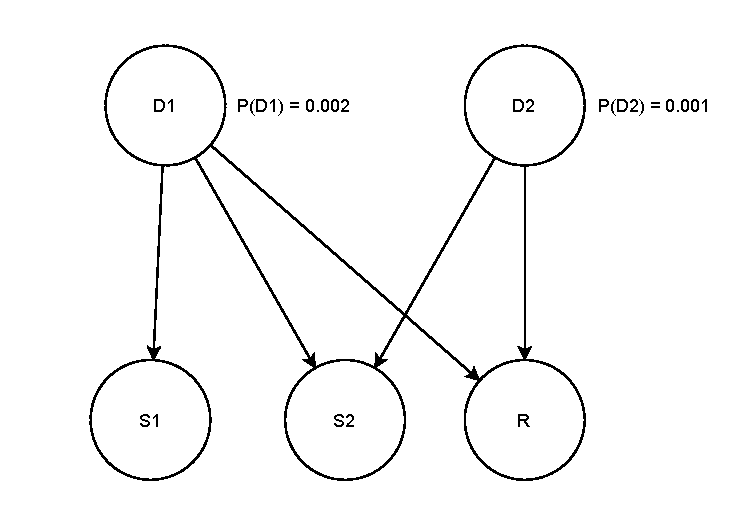
\includegraphics[width=0.99\linewidth]{arbolred.pdf}
  \end{center}
\end{figure}

Probabilidades asociadas a la red bayesiana:

\begin{center}
  \begin{tabular}{| c | c |}
    \hline
    \textbf{D1} & \textbf{P(S1/D1)} \\ \hline
    T & 0.7 \\ \hline
    F & 0.05 \\ \hline    
  \end{tabular}
\end{center}


\begin{center}
  \begin{tabular}{| c | c | c |}
    \hline
    \textbf{D1} & \textbf{D2} & \textbf{P(S2 / D1, D2)} \\ \hline
    T & T & 0.95 \\ \hline
    T & F & 0.2 \\ \hline
    F & T & 0.8 \\ \hline
    F & F & 0.05 \\ \hline    
  \end{tabular}
\end{center}

\begin{center}
  \begin{tabular}{| c | c | c |}
    \hline
    \textbf{D1} & \textbf{D2} & \textbf{P(R / D1, D2)} \\ \hline
    T & T & 0.5 \\ \hline
    T & F & 0.5 \\ \hline
    F & T & 0.5 \\ \hline
    F & F & 0 \\ \hline    
  \end{tabular}
\end{center}

Mediante este tipo de red se pueden representar las dependencias que existen
entre cierto conjunto de variables, permitiendo especificar de manera intutiva
la distribución de la probabilidad conjunta. Un ejemplo podría ser, en una fábrica
las probabilidades de encontrar fallas o defectos en ciertas piezas mecánicas según
en qué máquinas se manufacturen.


\subsection*{Apartado b)}

\begin{align*}
P(D1, \lnot D2, S1, R, \lnot S2) &= P(D1) P(\lnot D2) P(S1 / D1) P(R / D1, \lnot D2) P (\lnot S2 / D1, \lnot D2) \\
&= 0.002 * 0.999 * 0.7 * 0.5 * 0.8 \\
&= 0.00055944
\end{align*}

La probabilidad hallada es 0.00055944.

\subsection*{Apartado c)}

\begin{align*}
P(D2 / R, S2,\lnot S1) 
&= \frac{\displaystyle\sum_{x \in \{D1, \lnot D1\}} P(D2, R, S2, \lnot S1, x)}{\displaystyle\sum_{x \in \{D1, \lnot D1\} y \in \{D2, \lnot D2\}} P(R, S2, \lnot S1, x, y)} \\ \\
&= \frac{0.000000285 + 0.00037924}{0.000000285 + 0.00037924 + 0.00005994 + 0} \\ \\
&= \frac{0.000379525}{0.000439465} \\ \\
&= 0.863606886
\end{align*}

\begin{align*}
P(D1 / R, S2,\lnot S1) 
&= \frac{\displaystyle\sum_{x \in \{D2, \lnot D2\}} P(D1, R, S2, \lnot S1, x)}{\displaystyle\sum_{x \in \{D1, \lnot D1\} y \in \{D2, \lnot D2\}} P(R, S2, \lnot S1, x, y)} \\ \\
&= \frac{0.000000285 + 0.00005994}{0.000439465} \\ \\
&= 0.1370416302
\end{align*}

El paciente presenta una probabilidad muy alta (aprox. 86\%) de tener la enfermedad D2.

\end{document}